\subsection{DNF}

\begin{definition}
    Dysjunktywna postać normalna (DNF -- disjunctive normal form) formuły boolowskiej to postać, która jest alternatywą klauzul składających się z koniunkcji literałów, np.
    \[ \left( x_1 \land \overline{x_2} \land x_2 \right) \lor \left( \overline{x_1} \land x_3 \right) \lor \left( \overline{x_1} \land \overline{x_2} \land x_4 \land x_5 \right) . \] 
    Łatwo jest sprawdzić, czy taka formuła jest spełnialna -- wystarczy, że jakaś formuła nie zawiera wyrażenia postaci \(x \land \overline{x}\).
\end{definition}

    Chcemy znaleźć FPRAS dla problemu zliczenia wartościowań spełniających formułę logiczną \(F\) o \(n\) zmiennych. Oznaczmy tę wartość przez \(C\left( F \right) \) i zdefiniujmy \(R\left( F \right) = \frac{C\left( F \right) }{2^{n}}\). Możemy podejść do sprawy naiwnie: losujemy jednostajnie wartościowanie i oznaczamy przez \(X\) indykator tego, czy spełnia ono \(F\). Mamy \(\mathbb{\mathbb{E}}\left[ X \right] = R\left( F \right) \) i po powtórzeniu eksperymentu \(m \ge \frac{3 \ln\left( \frac{2}{\delta} \right) }{R\left( F \right) \varepsilon^2}\) razy dostaniemy \(\left( \varepsilon, \delta \right) \)-aproksymację. Wartość \(\frac{1}{R\left( F \right) }= \frac{2^{n}}{C\left( F \right) }\) jest wielomianowa od \(n\) dla \(C\left( F \right) = \frac{2^{n}}{\mathrm{poly}\left( n \right) }\), ale dla mniejszych już niekoniecznie. Zatem przedstawione podejście nie zawsze daje nam FPRAS.

\begin{theorem}
    Mając zadaną formułę w postaci DNF \(F = C_1 \lor C_2 \lor \ldots\lor C_t\) o \(n\) zmiennych możemy wyznaczyć liczbę wartościowań ją spełniających \(C\left( F \right) \) za pomocą następującego algorytmu: pozbywamy się klauzul zawierających wyrażenia postaci \(x \land \overline{x}\) i definiujemy \(SC_i\) jako zbiór wartościowań spełniających \(C_i\). Do tego \(S = \left\{ \left( i,a \right) : i \in [t], a \in SC_i \right\} \), \(RC_i = SC_i \setminus \bigcup_{j=1}^{i-1} SC_j\), \(R = \left\{ \left( i,a \right) : i \in [t], a \in RC_i \right\} \).

    Wybieramy \(i \in [t]\) z prawdopodobieństwem \(\frac{\left|SC_i\right|}{\left|S\right|}\) a następnie wybieramy jednostajnie wartościowanie \(a \in SC_i\). Niech \(X\) będzie indykatorem tego, czy \(a \in RC_i\). Mamy \(\mathbb{\mathbb{E}}\left[ X \right] = \frac{C\left( F \right) }{\left|S\right|}\) i taki algorytm daje nam FPRAS.
\end{theorem}
\begin{proof}
    Zauważmy, że pozbycie się klauzul zawierających \(x \land \overline{x}\) można wykonać liniowym przejściem po klauzulach. Jeśli \(C_i\) ma \(\ell_i\) literałów (czyli \(\ell_i\) zmiennych), to spełnia ją dokładnie \(2^{n-\ell_i}\) wartościowań (ustalamy zmienne w klauzuli, reszta dowolnie). Mamy \(\left|S\right|= \sum_{i=1}^{t} \left|SC_i\right| = \sum_{i=1}^{t} 2^{n-\ell_i}\), a więc tę liczbę da się łatwo wyznaczyć. \(RC_i\) jest zbiorem wartościowań, które spełniają \(C_i\), ale nie spełniają żadnej poprzedniej klauzuli. Jasne, że \(C\left( F \right) = \left|R\right|\) (każde wartościowanie liczymy raz). Nasz algorytm właściwie losuje parę \(\left( i,a \right) \in S\) i sprawdza, czy \(\left( i,a \right) \in R \). Co więcej, robi to jednostajnie: najpierw wybieramy \(i\) z prawdopodobieństwem \(\frac{\left|SC_i\right|}{\left|S\right|}\), a następnie \(a\) z prawdopodobieństwem \(\frac{1}{\left|SC_i\right|}\) -- razem \(\frac{1}{\left|S\right|}\). Zauważmy, że wylosowanie \(a\) da się zrobić łatwo -- losujemy jednostajnie wartości literałów nie ustalonych przez \(C_i\). Dla \(R\left( F \right) = \frac{C\left( F \right) }{\left|S\right|} = \frac{\left|R\right|}{\left|S\right|}\) mamy \(\mathbb{\mathbb{E}}\left[ X \right] = R\left( F \right) \). Aby dostać \(\left( \varepsilon, \delta \right) \)-aproksymację musimy powtórzyć losowanie \(\frac{3\ln\left( \frac{2}{\delta} \right) }{R\left( F \right) \varepsilon^2}\) razy. Mamy \(\frac{1}{R\left( F \right) } = \frac{\left|S\right|}{\left|R\right|} \le t \), bo każde wartościowanie z \(R\) występuje w \(S\) co najwyżej \(t\) razy. Zatem \(\frac{1}{R\left( F \right) }\) jest wielomianowe od \(F\) i faktycznie mamy FPRAS.
\end{proof}

\subsection{FPRAS z FPAUS}

\begin{theorem}
    Niech \(\Omega\left( G  \right) \) oznacza rodzinę zbiorów niezależnych w grafie \(G\). Zakładając, że mamy dla niej FPAUS, istnieje FPRAS jej rozmiaru.
\end{theorem}
\begin{proof}
    Będziemy chcieli znaleźć \(\left( \varepsilon,\delta \right) \)-aproksymację \(\left|\Omega\left( G  \right) \right|\). Ustalamy porządek \(e_1,\ldots,e_k\) na krawędziach \(G\) i oznaczamy \(G_i = \left( V\left( G  \right) , \left\{ e_1,\ldots,e_i \right\}  \right) \). \(G_0\) nie ma krawędzi, a więc \(\left|\Omega\left( G_0 \right) \right|= 2^{n}\), gdzie \(n = \left|V\left( G  \right) \right|\). Do tego \(G_k = G \). Niech  \(r_i = \frac{\left|\Omega\left( G_i \right) \right|}{\left|\Omega\left( G_{i-1} \right) \right|}\),  \(\varepsilon' = \frac{\varepsilon}{2k}\), \(\delta' = \frac{\delta}{k}\).

    Zauważmy, że mamy \(\left|\Omega\left( G  \right) \right|= \frac{\left|\Omega\left( G_k \right) \right|}{\left|\Omega\left( G_{k-1} \right) \right|}\cdot \ldots\cdot \frac{\left|\Omega\left( G_1 \right) \right|}{\left|\Omega\left( G_0 \right) \right|}\cdot \left|\Omega\left( G_0 \right) \right| = r_k\cdot \ldots\cdot r_1\cdot 2^{n}\). Będziemy chcieli znaleźć \(s_i\) będące \(\left( \varepsilon',\delta' \right) \)-aproksymacją \(r_i\). Niech \(W = s_k\cdot \ldots\cdot s_1\cdot 2^{n}\). Mając \(P\left( \left|s_i-r_i\right|> \varepsilon' r_i \right) < \delta'\) dostajemy
    \[ P\left( \bigcup_{i=1}^{k} \left\{ \left|s_i-r_i\right|> \varepsilon' r_i \right\}  \right) \le \sum_{i=1}^{k} P\left( \left|s_i-r_i\right|> \varepsilon' r_i \right) < k\cdot \delta' = \delta. \] 
    Teraz możemy przeliczyć
    \begin{align*}
        &P\left( \left|W - \left|\Omega\left( G \right) \right| \right|\le \left|\Omega\left( G  \right) \right|\varepsilon \right) = P\left( 1-\varepsilon \le \frac{W}{\left|\Omega\left( G  \right) \right|}\le 1+\varepsilon  \right) = P\left( 1-\varepsilon \le \prod_{i=1}^{k} \frac{s_i}{r_i} \le 1+\varepsilon   \right) \ge \\ 
        &P\left( \bigcap_{i=1}^{k} \left\{ 1 - \varepsilon' \le \frac{s_i}{r_i} \le 1+\varepsilon' \right\}  \right) = P\left( \bigcap_{i=1}^{k} \left\{ \left|s_i-r_i\right|\le \varepsilon' r_i \right\}  \right) \ge 1-\delta,
    \end{align*}
    gdzie pierwsza nierówność jest konsekwencją ciągu nierówności
    \[ 1-\varepsilon \le \left( 1-\frac{\varepsilon }{2k} \right) ^{k} \le \prod_{i=1}^{k} \frac{s_i}{r_i} \le \left( 1+\frac{\varepsilon }{2k} \right) ^{k} \le 1+\varepsilon.  \] 
    Pierwsza z tych nierówności wynika z nierówności Bernoulliego \(\left( 1-\frac{\varepsilon }{2k} \right) ^{k} \ge 1-\frac{\varepsilon }{2}\), a ostatnia to szacowanie \(\left( 1+\frac{\varepsilon }{2k} \right) ^{k} = \sum_{i=0}^{k} \binom{k}{i} \left( \frac{\varepsilon }{2k} \right) ^{i} \le \sum_{i=0}^{k} k^{i} \frac{\varepsilon^{i}}{2^{i}k^{i}} \le 1+ \sum_{i=1}^{k} \frac{\varepsilon }{2^{i}} \le 1+\varepsilon\), gdzie w przedostatnim kroku założyliśmy \(\varepsilon \le 1\).

    Z tego wynika, że jeśli znajdziemy FPRAS dla wartości \(R = \frac{\left|\Omega\left( H  \right) \right|}{\left|\Omega\left( H' \right) \right|}\), gdzie \(H = H' + e\) dla pewnej krawędzi \(e\), to uzyskamy naszą tezę. Wykorzystamy do tego FPAUS. Bierzemy \(\frac{\varepsilon'}{3}\)-jednostajnie zbiór \(I \in \Omega\left( H' \right) \) i ustalamy indykator \(X = \left[ I \in \Omega\left( H  \right)  \right] \). Powtarzamy taki eksperyment \(m\) razy: \(Y = \frac{1}{m} \sum_{i=1}^{m} X_i\). Niech \(\mu = \mathbb{E}\left[ Y \right] \).

    Zauważmy, że mamy \(R \ge \frac{1}{2}\) -- każdy zbiór niezależny w \(\Omega\left( H' \right) \setminus \Omega\left( H  \right) \) można jednoznacznie przypisać do zbioru w \(\Omega\left( H  \right) \) odejmując od niego \(v\) będące ustalonym końcem \(e\). Zatem w \(\Omega\left( H' \right) \) jest co najwyżej dwa razy więcej zbiorów. Z określenia naszego próbkowania mamy \(\left|\mu - R \right|= \left|P\left( I \in \Omega\left( H  \right)  \right) - R \right|\le \frac{\varepsilon'}{3}\). Z tego mamy \(\mu \ge \frac{1}{3}\), bo można założyć \(\varepsilon' \le \frac{1}{2}\). Do tego
    \[ 1-\frac{2\varepsilon'}{3} \le 1-\frac{\varepsilon'}{3R} \le \frac{\mu}{R} \le 1+\frac{\varepsilon'}{3R} \le 1+\frac{2\varepsilon'}{3}. \] 
    Biorąc \(m \ge \frac{9\ln\left( \frac{2}{\delta'} \right) }{\left( \frac{\varepsilon'}{6} \right) ^{2}}\ge \frac{3 \ln\left( \frac{2}{\delta'} \right) }{\mu \left( \frac{\varepsilon'}{6} \right) ^2} \) dostajemy z nierówności Czernowa \(P\left( 1-\frac{\varepsilon'}{6}\le \frac{Y}{\mu} \le 1+\frac{\varepsilon'}{6} \right) \ge 1-\delta'\). W połączeniu z poprzednim daje nam to
    \[ P\left( \left( 1-\frac{\varepsilon'}{6} \right) \left( 1-\frac{2\varepsilon'}{3} \right) \le \frac{Y}{\mu}\cdot \frac{\mu}{R} \le \left( 1+\frac{\varepsilon'}{6} \right) \left( 1+\frac{2\varepsilon'}{3} \right)\right) \ge 1-\delta'. \] 
    Rozpisując lewą stronę nierówności dostajemy 
     \[ \left( 1-\frac{\varepsilon'}{6} \right) \left( 1-\frac{2\varepsilon'}{3} \right) = 1 - \frac{5\varepsilon'}{6} + \frac{\varepsilon'^2}{9} \ge 1-\varepsilon' \] 
     i podobnie dla prawej strony. Mamy zatem
     \[ P\left( 1-\varepsilon' \le \frac{Y}{R} \le 1+\varepsilon' \right) \ge 1-\delta', \] 
     czyli przedstawiony proces daje dobrą aproksymację \(R\). Zauważmy jeszcze, że \(m\) jest wielomianowe od wejścia, a więc mamy FPRAS.
\end{proof}

\subsection{FPAUS ze sprzęgania}

\begin{theorem}
    Rozważmy graf \(G\) z \(\Delta\left( G  \right) \le 4\), w którym do tego nie ma trójkątów (W książce \textit{Probability and Computing} nie ma tego założenia. Jest ono jednak potrzebne w części dowodu, w której rozważamy przypadki.). Niech \(\Omega\left( G  \right) \) będzie rodziną zbiorów niezależnych w \(G\). Istnieje FPAUS dla \(\Omega\left( G  \right) \).
\end{theorem}
\begin{proof}
    Możemy założyć bez straty ogólności, że \(G\) jest spójny -- inaczej można próbkować z każdej składowej osobno. Zdefiniujemy łańcuch Markowa o stanach z \(\Omega\left( G  \right) \) w następujący sposób: jego krok \(K^{p}_{e}\left( I \right) \) polega na wylosowaniu jednostajnie \(e = uv\) z \(\mathbb{E}\left( G  \right) \) (ustalamy jakiś porządek na wierzchołkach, żeby móc mówić o pierwszy i drugim wierzchołku krawędzi) i \( p \in \left\{ 1,2,3 \right\} \). Teraz mamy przypadki
    \[ \begin{array}{l} p = 1 \to I' = I\setminus \left\{ u,v \right\} \\ p =2 \to I' = I\setminus \left\{ u  \right\} \cup \left\{ v  \right\} \\ p=3 \to I' = I\setminus \left\{ v  \right\} \cup \left\{ u  \right\}  \end{array} .\] 
    Jeśli \(I' \in \Omega\left( G  \right) \), to \(K^{p}_{e}\left( I  \right) = I'\), inaczej \(K^{p}_{e}\left( I  \right) = I \). Tak zadany łańcuch jest nieprzywiedlny i nieokresowy -- można usuwać odpowiednie wierzchołki aż osiągnie się zbiór pusty, a potem dodawać odpowiednie wierzchołki i otrzymać dowolny zbiór. Nieokresowość wynika z tego, że można stać w miejscu. Rozkład stacjonarny tego łańcucha jest jednostajny, bo prawdopodobieństwo przejścia \(I\to J\) jest takie samo jak \(J \to I \).

    Rozważmy sprzęganie \(\left( \left( X_t,Y_t \right)  \right) _{t \in \N}\) łańcuchów takie, że w kroku losujemy jednostajnie \(p_t,e_t\) i ustalamy \(\left( X_{t+1},Y_{t+1} \right) = \left( K_{e_t}^{p_t}\left( X_t \right) , K_{e_t}^{p_t}\left( Y_t \right)  \right) \). Skracamy zapis \(K = K_{e_t}^{p_t}\). Oznaczmy \(d_t = \left|X_t \Delta Y_t\right|\), gdzie \(\Delta\) oznacza różnicę symetryczną. Pokażemy, że \(\mathbb{E}\left[ d_{t+1}\mid d_t \right] \le d_t\). Zwykle wykazywaliśmy ostrą nierówność i z niej wynikało ograniczenie na czas mieszania. Z nieostrej też wynika szybkie mieszanie się łańcucha, ale nie będziemy tego pokazywać.

    Jeśli \(d_t = 0\), to \(d_{t+1}=0\). Rozważmy teraz przypadek \(d_t = 1\) -- mamy \(I,J \in \Omega\left( G  \right) \) takie, że \(J = I \cup \left\{ x  \right\} \) i chcemy pokazać, że dla \(D = \left|K\left( I  \right) \Delta K\left( J \right) \right|\) zachodzi \(\mathbb{E}\left[ D  \right] \le 1\). Niech \(e = uv\). Jeśli \(u,v \notin N\left( x  \right) \), to \(D = 1\), bo oba zbiory zachowają się tak samo podczas przejścia. Załóżmy, że \(u \in N\left( x  \right) \). Skorzystamy teraz z założeń i rozpatrzymy przypadki.
    \begin{enumerate}
        \item \(\left|N\left( u  \right) \cap I \right|\ge 2\). Tutaj zawsze \(D \le 1\), co sprawdzamy rozpatrując wszystkie przypadki.
        \item \(\left|N\left( u  \right) \cap I \right|= 1\). Patrząc na rysunek: jeśli \(v \in \left\{ v_2,v_3 \right\} \), to \(D = 1\), bo w obu zbiorach zrobimy to samo (m.in. tu ważny jest brak trójkątów -- \(v\) nie jest połączone z \(x\)). Jeśli \(v = x \), to \(p \in \left\{ 1,2 \right\}  \to  D=0\) (usuwamy albo dodajemy \(x\) do obu) a \(p = 3 \to D = 1\), bo ruch się nie uda. Jeśli \(v = v_1\), to \(p \in \left\{ 1,2 \right\} \to D=1\), ale \(p=3 \to D=3\), bo ruch nie uda się dla \(J\), ale uda się dla \(I\). Widzimy, że wartość oczekiwana  \(D\) w tej sytuacji to \(1\).
        \item \(\left|N\left( u  \right) \cap I \right|=0\). Jeśli \(v=x\), to \(D=0\). Jeśli \(v = v_i\) dla \(v_i \in N\left( u  \right) \setminus \left\{ x \right\} \), to \(p \in \left\{ 1,2 \right\} \to D=1\), ale \(p=3 \to D=2\), bo \(u\) zostanie dodane do \(I\). Mamy 
    \[\mathbb{E}\left[ D \mid e \in \left\{ ux, uv_i \right\}  \right] \le \frac{1}{\Delta\left( G  \right) }\cdot 0 + \frac{\Delta\left( G  \right) -1}{\Delta\left( G  \right) }\left( \frac{2}{3}\cdot 1 + \frac{1}{3}\cdot 2 \right) = \frac{\Delta\left( G  \right) -1}{\Delta\left( G  \right) }\cdot \frac{4}{3}\le 1.\]
    \end{enumerate}
\begin{figure}[H]
    \centering
    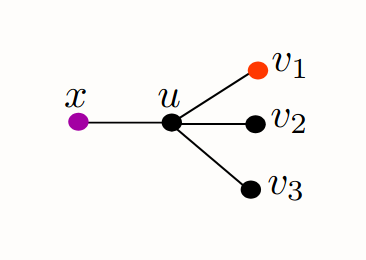
\includegraphics{img/monte-carlo/neighbours.png}
    \caption{Przypadek, gdy \(I\) ma w sobie jednego sąsiada \(u\).}
    \label{fig:path-coupling}
\end{figure}
    Pozostało nam rozważyć przypadek \(d_t > 1\). Zastosujemy metodę path coupling -- połączymy \(X_t\) z \(Y_t\) ,,ścieżką''. Niech \(X_t \setminus Y_t = \left\{ x_1,\ldots,x_r \right\} \), \(Y_t \setminus X_t = \left\{ y_1,\ldots,y_s \right\} \). Oznaczmy 
    \[Z_0 = X_t, Z_1 = X_t \setminus \left\{ x_1 \right\} ,\ldots, Z_r = X_t \cap Y_t, Z_{r+1} = \left( X_t \cap Y_t \right) \cup \left\{ y_1 \right\} ,\ldots, Z_{r+s} = Z_{d_t} = Y_t .\]
    Mamy \(\left|Z_{i-1}\Delta Z_i\right|=1\), a więc \(\mathbb{E}\left[ \left|K\left( Z_{i-1} \right) \Delta K\left( Z_i \right) \right| \right] \le 1\). Korzystając z nierówności \(\left|A\setminus B \right|\le \left|A\setminus C \right|+\left|C\setminus B\right|\) dostajemy
    \[ \left|K\left( Z_0 \right) \setminus K\left( Z_{d_t} \right) \right|\le \left|K\left( Z_0 \right) \setminus K\left( Z_1 \right) \right|+ \left|K\left( Z_1 \right) \setminus K\left( Z_{d_t} \right) \right|\le \ldots\le \sum_{i=1}^{d_t} \left|K\left( Z_{i-1} \right) \setminus Z_i\right|, \] 
    a więc
    \begin{align*}
        &\left|K\left( Z_0 \right) \Delta K\left( Z_{d_t} \right) \right| = \left|K\left( Z_0 \right) \setminus  K\left( Z_{d_t} \right) \right|+ \left|K\left( Z_{d_t} \right) \setminus K\left( Z_0 \right) \right| \\ 
        &\le \sum_{i=1}^{d_t} \left|K\left( Z_{i-1} \right) \setminus K\left( Z_i \right) \right|+ \left|K\left( Z_i \right) \setminus K\left( Z_{i-1} \right) \right| = \sum_{i=1}^{d_t} \left|K\left( Z_{i-1}\right) \Delta K\left( Z_i \right)  \right| .
    \end{align*}
    To daje nam
    \[ d_{t+1} = \left|X_{t+1}\Delta Y_{t+1}\right| = \left|K\left( Z_0 \right) \Delta K\left( Z_{d_t} \right) \right|\le \sum_{i=1}^{d_t} \left|K\left( Z_{i-1} \right) \Delta K\left( Z_i \right) \right|. \] 
    Ostatecznie
    \[ \mathbb{E}\left[ d_{t+1} \mid d_t \right] \le \sum_{i=1}^{d_t} \mathbb{E}\left[ \left|K\left( Z_{i-1} \right) \Delta K\left( Z_i \right) \right| \right] \le d_t. \] 
\end{proof}

